\chapter{Introduction} \label{ch:Introduction}
%Here comes the introduction. Explain why the topic of your thesis is important and what is the goal of the thesis. If you need, use references like this \cite{higham2020handbook}. If you want to use acronyms, define a \textit{newacronym} in the file "sybol\_directory.tex" and use it like this: \gls{lti}. The next time you use the acronym \gls{lti} is appears authomatically in short form.  
%
%You can also include images like this.
%\begin{figure}[ht!]
%    \centering
%    
\includegraphics[width=\textwidth]{03_images/meme.png}
%    \caption{Graphical representation of the research process.}
%    \label{fig:Introduction:meme}
%\end{figure}
%
%
%A meme can be seen in Figure~\ref*{fig:Introduction:meme}. This demonstrates that 
%\begin{equation} \label{eq:Introduction:realisation}
%	1 \le 2 \ \text{or} \ 1 \ge 2.
%\end{equation}
%In addition to \eqref{eq:Introduction:realisation}, it could be postulated that $1 \ne 2$. Further discussions are considered in the following sections and subsections.
\newtheorem{definition}{Definition}
\section{Background and Motivation} \label{sec:Introduction:Background}
Robots are used extensively in the industrial production of automobiles, air- and spacecrafts, as well as the production of commodities.The rapid development of robotics makes robot applications in production more efficient and affordable \cite{EEUIR}. The cost difference compared to traditional products manufactured by traditional machines is becoming smaller \cite{IAP}. Traditional machine manufacturing is suitable for mass production of identical parts with limited or no variations \cite{IAP}. However, industrial robots possess flexibility due to their multiple degrees of freedom to tackle complex personalized production such as customized rims and furniture, to meet individual customer requirements \cite{IAP}. Robots tend to replace traditional machinings in such production branches with a higher degree of personalization, which can vastly improve economic efficiency and save energy \cite{EEUIR}.\par
The high demands of the production process, particularly in producing significant aircraft components, have created the need for multi-robot systems. Efficiency can be increased by letting multiple robots work simultaneously. Systems made up of multiple robots have the following advantages over an individual robot \cite{PFRCD} \cite{KMR}.
\begin{itemize}
 \item \textbf{High adaptability to the environment}: Compared to individual robots, multi-robot systems show greater flexibility and adaptability to tasks because such systems allow a better distribution in functionalities and space than individual robots.
 \item \textbf{High efficiency}: A multi-robot system is a group in which each robot works individually while coordinating with the others, thus significantly reducing working times and effectively increasing productivity.
 \item \textbf{High robustness}: In a multi-robot system, due to its redundancy, the system should still be able to function correctly when a few robots fail.
\end{itemize}
Industrial robots have evolved from traditional handling, assembly, and welding tasks to a wide range of production applications. The use of robots in manufacturing processes can lead to high flexibility and low costs \cite{IAP}. However, the performance of robots is hardly comparable to that of machine tools, such as absolute precision, manufacturing error, structural integrity under vibration etc. Stiffness is considered to be a significant weakness in robotic machining applications \cite{MIIR}.\par
As shown in Figure \ref{fig:Introduction:co_model} in manufacturing, two coupled robots provide higher stiffness than one robot \cite{VSK}. Intuitively, two coupled robots are like two parallel connected springs \cite{VSK}. To enhance manufacturing quality in robotic machining, physically coupled multi-robot systems are used. Physically coupled robots perform coordinated actions through force interactions. The end-effectors or flanges of several robots can be connected utilizing a rigid coupler. Physically coupled robots perform coordinated machining tasks. Various machining tasks, such as drilling and milling, can be implemented if tools are attached to the coupler. Most stiffness problems in robot-driven machining research have been on a single robot \cite{WPOIR} \cite{POMIR} \cite{SOPO}, and there is a need to extend the studies on optimizing robot stiffness in manufacturing processes.\par
\begin{figure}[h!]
	\centering
	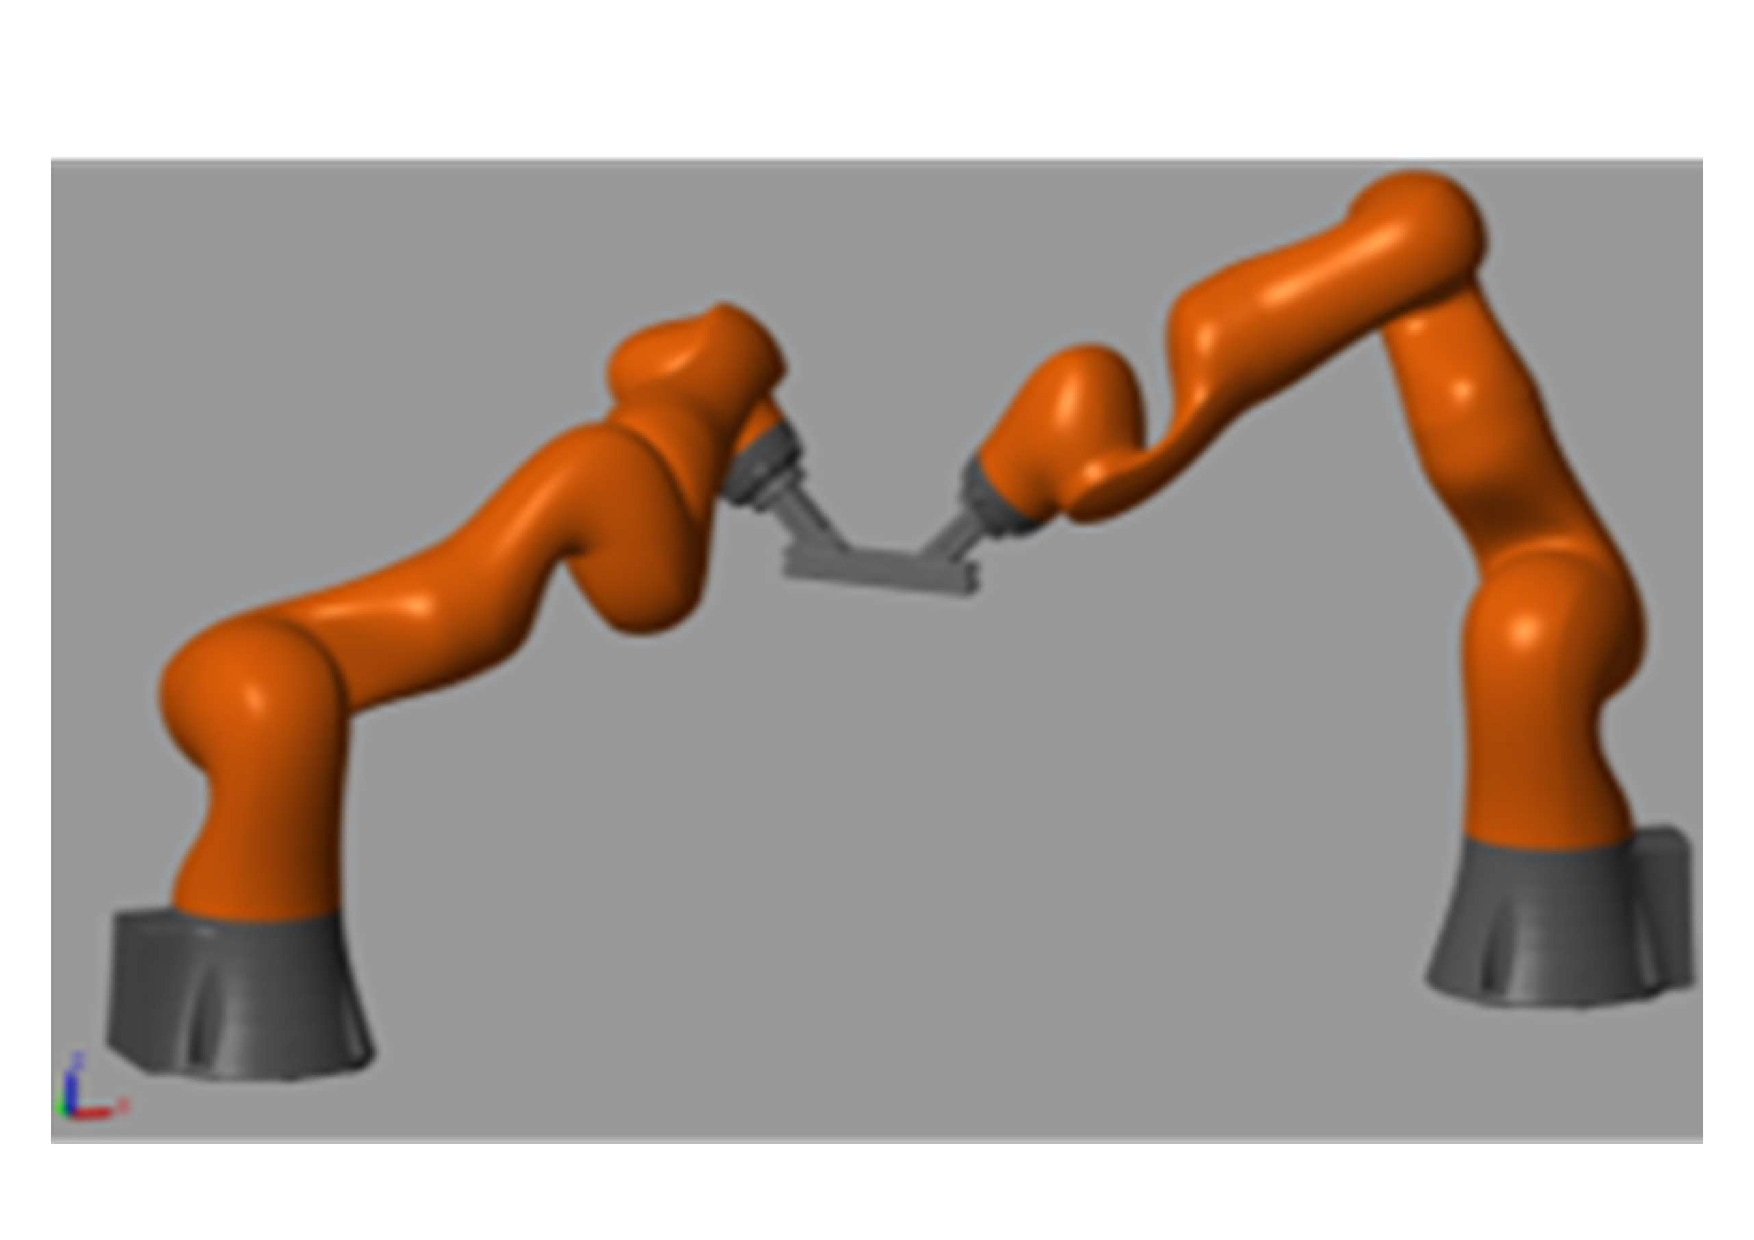
\includegraphics[width=6cm]{03_images/co_model.pdf}
	\caption{The Model of coupled robots}
	\label{fig:Introduction:co_model}
\end{figure}

In summary, to enhance robot manufacturing quality, it is necessary to enhance the stiffness of the coupled robot. The challenges of enhancing stiffness are as follows:\par
(1)Finding stiff configurations along the whole path, but not on a single point.\par
(2)Keeping the robots coupled while searching for a stiffer pose.\par
(3)Generating smooth robot movements.\par

%\subsection{Contribution of my thesis}
%
%text text text text text text text text text text text text text text text text text text text text text text text text text text text text text text text text text text text text text text text 

\section{Problem Definition} \label{sec:Introduction:Problem Definition}
The stiffness is defined before a precise definition of the problem is given.\par
\begin{definition}[Stiffness]
	Stiffness is the extent to which an object resists deformation in response to an applied force. \cite{swms}
\end{definition}
\begin{equation} \label{equ:Hooke}
F =  kx
\end{equation}
Formula \ref{equ:Hooke} is Hooke’s Law: $F$ means Force, $x$ means displacement, and $k$ means stiffness.\par
\begin{figure}[h!]
	\centering
	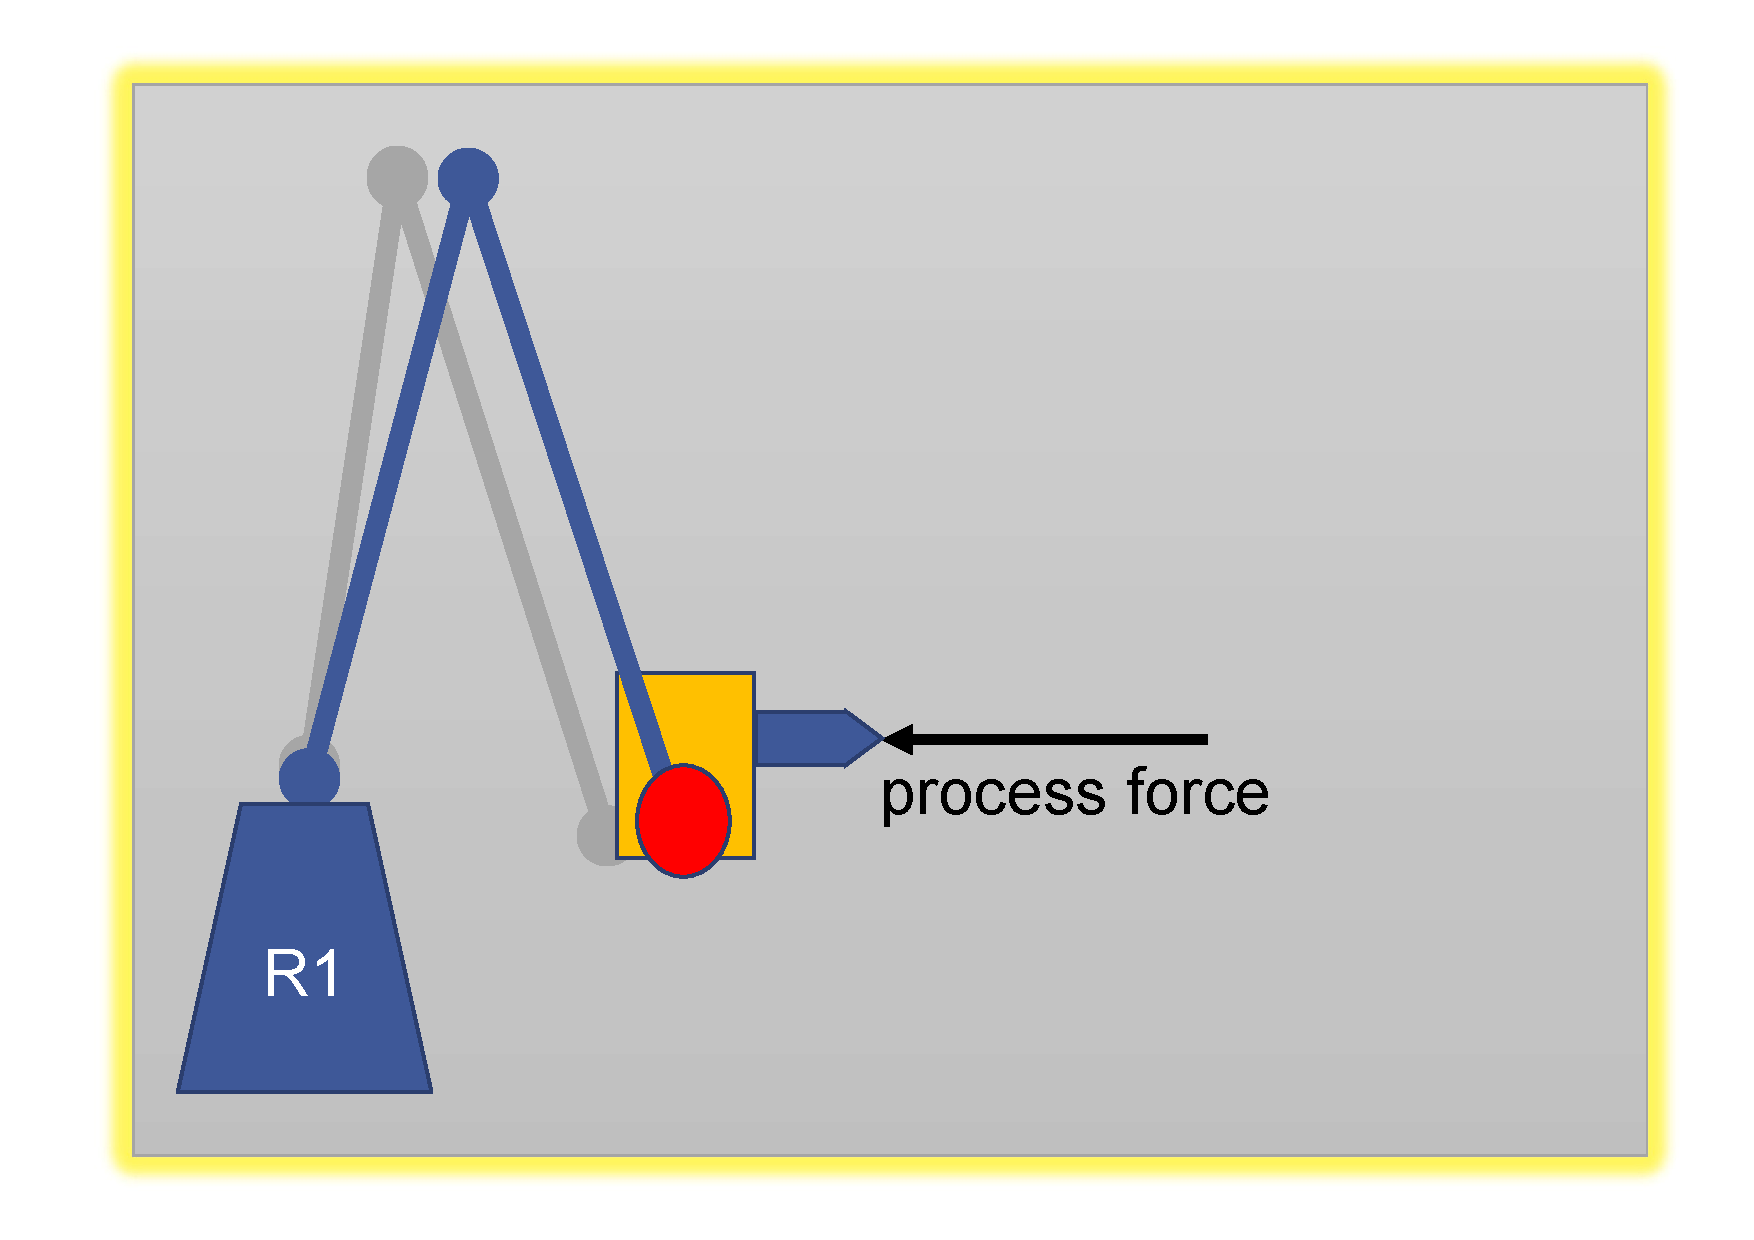
\includegraphics[width=6cm]{03_images/stiff.pdf}
	\caption{Deformation of the robot arm}
	\label{fig:Introduction:stiff}
\end{figure}
The robotic arm is deformed when a process force is applied to its end effector, as shown in Figure \ref{fig:Introduction:stiff}, changing from the blue pose to the light grey pose. Stiffness is considered an essential weakness in robotic machining processes, so it is important to increase the stiffness to meet quality requirements \cite{WPOIR}.\par
With the enhanced stiffness, the manufacturing error in machining is reduced. As shown different stiffness levels in the following two pictures, stiffness in Figure \ref{fig:Introduction:configuration1} with asymmetrical configuration has enhanced compared to in Figure \ref{fig:Introduction:configuration2} with conservative configuration.\par
\begin{figure}[h!]
\centering
\begin{minipage}[t]{0.48\textwidth}
\centering
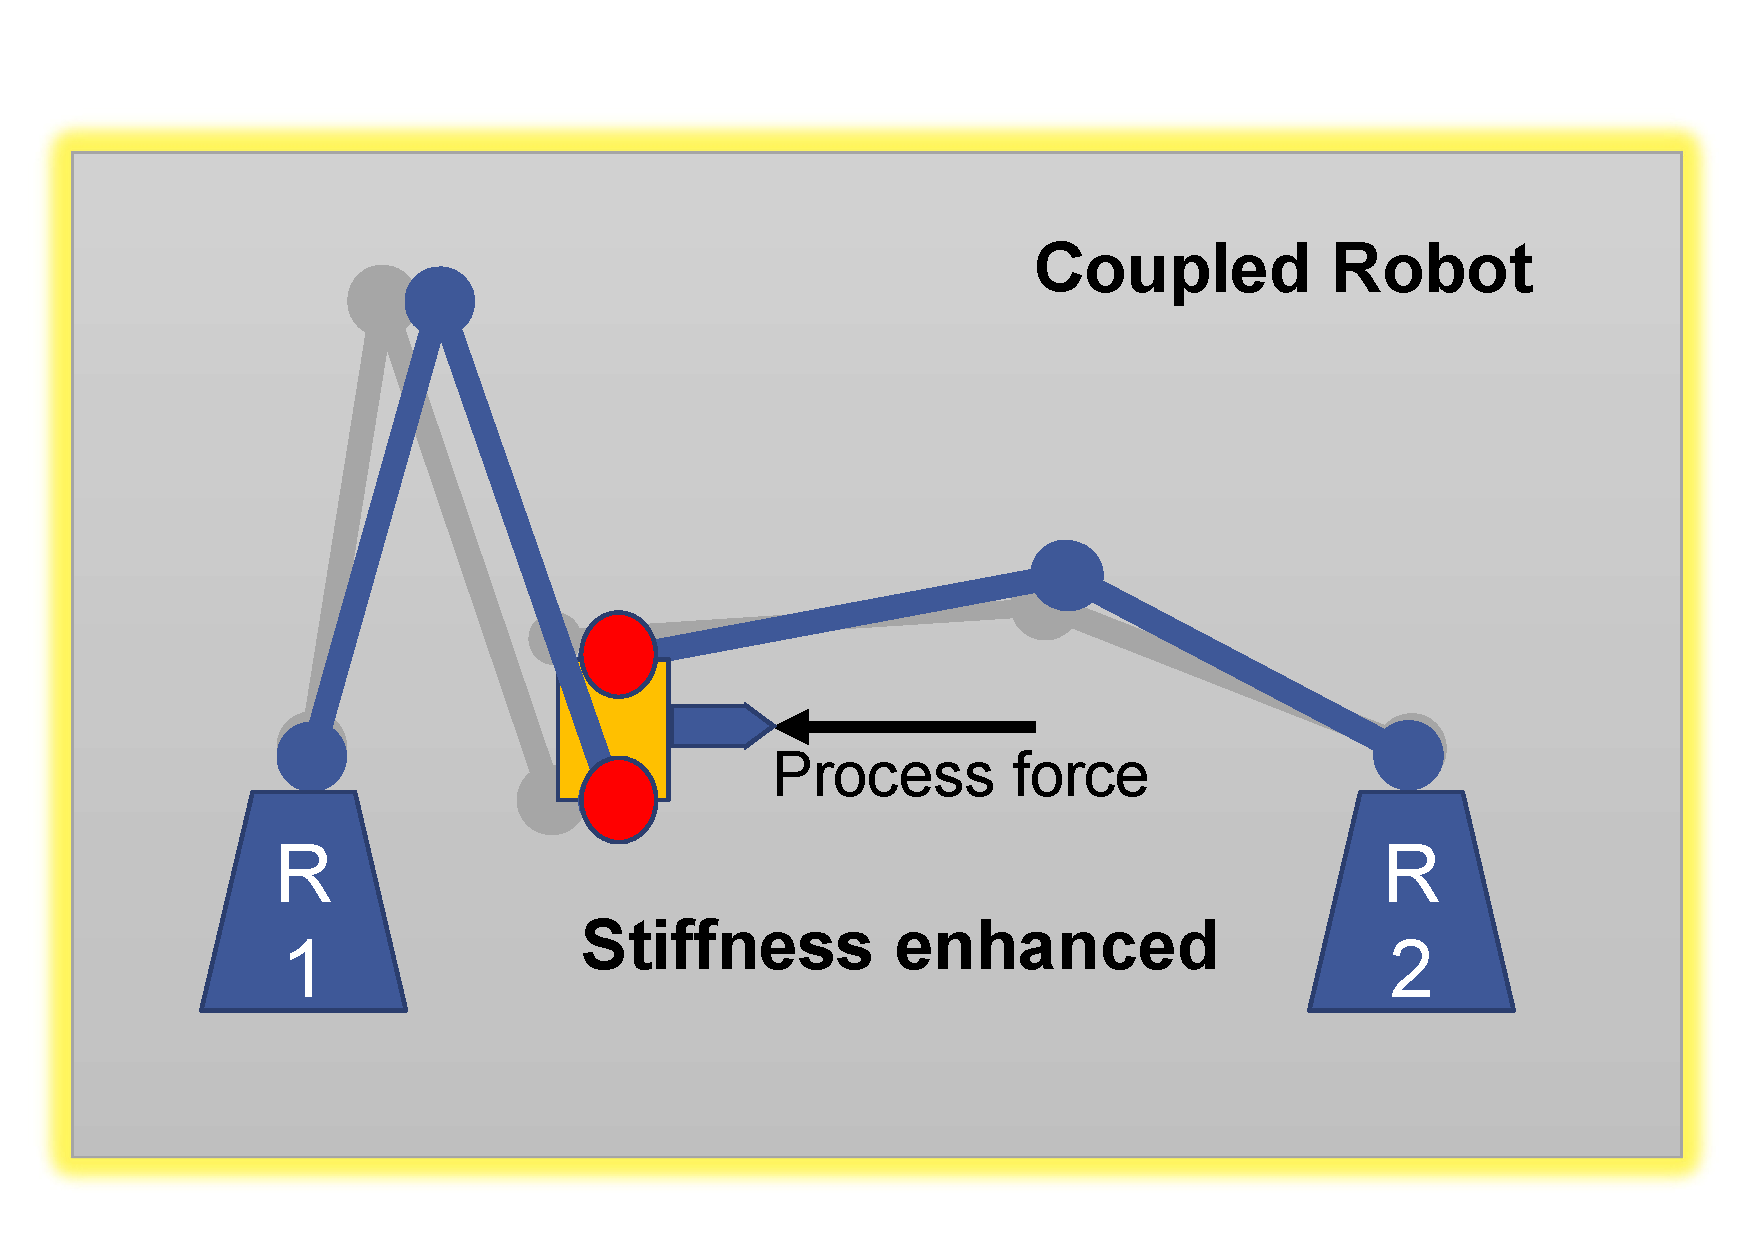
\includegraphics[width=6cm]{03_images/co_stiff_1.pdf}
\caption{Configuration 1}
\label{fig:Introduction:configuration1}
\end{minipage}
\begin{minipage}[t]{0.48\textwidth}
\centering
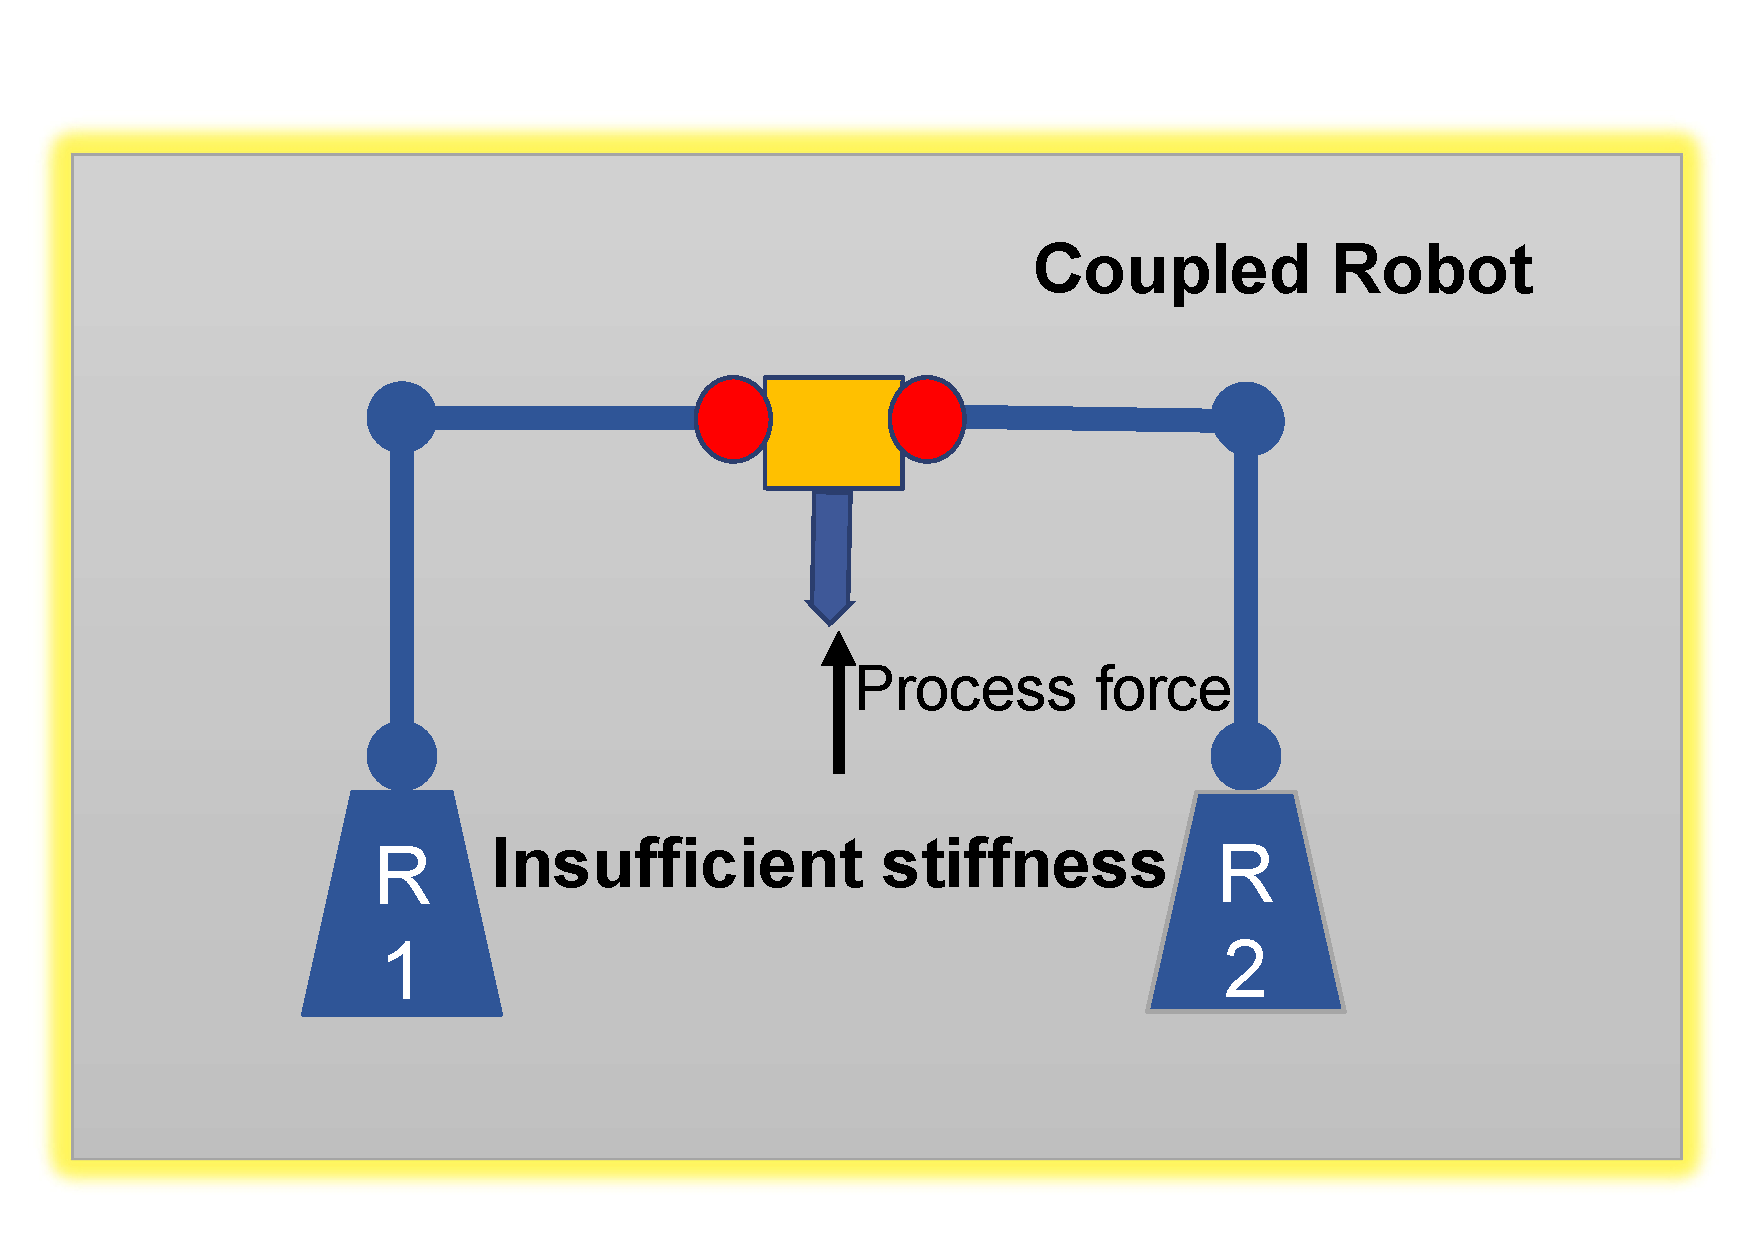
\includegraphics[width=6cm]{03_images/co_stiff_2.pdf}
\caption{Configuration 2}
\label{fig:Introduction:configuration2}
\end{minipage}
\end{figure}
In addition, the placement of the workpiece is also an influencing factor that the end effector needs to reach a different position due to the different placement of the workpiece, resulting in a different joint angle configuration of the coupled robot, which also changes the stiffness of the coupling robot during the machining process.\par
In summary, the factors influencing the stiffness of the coupling robot are the joint angle configuration and the corresponding placement of the workpiece.\par
\begin{figure}[ht!]
	\centering
	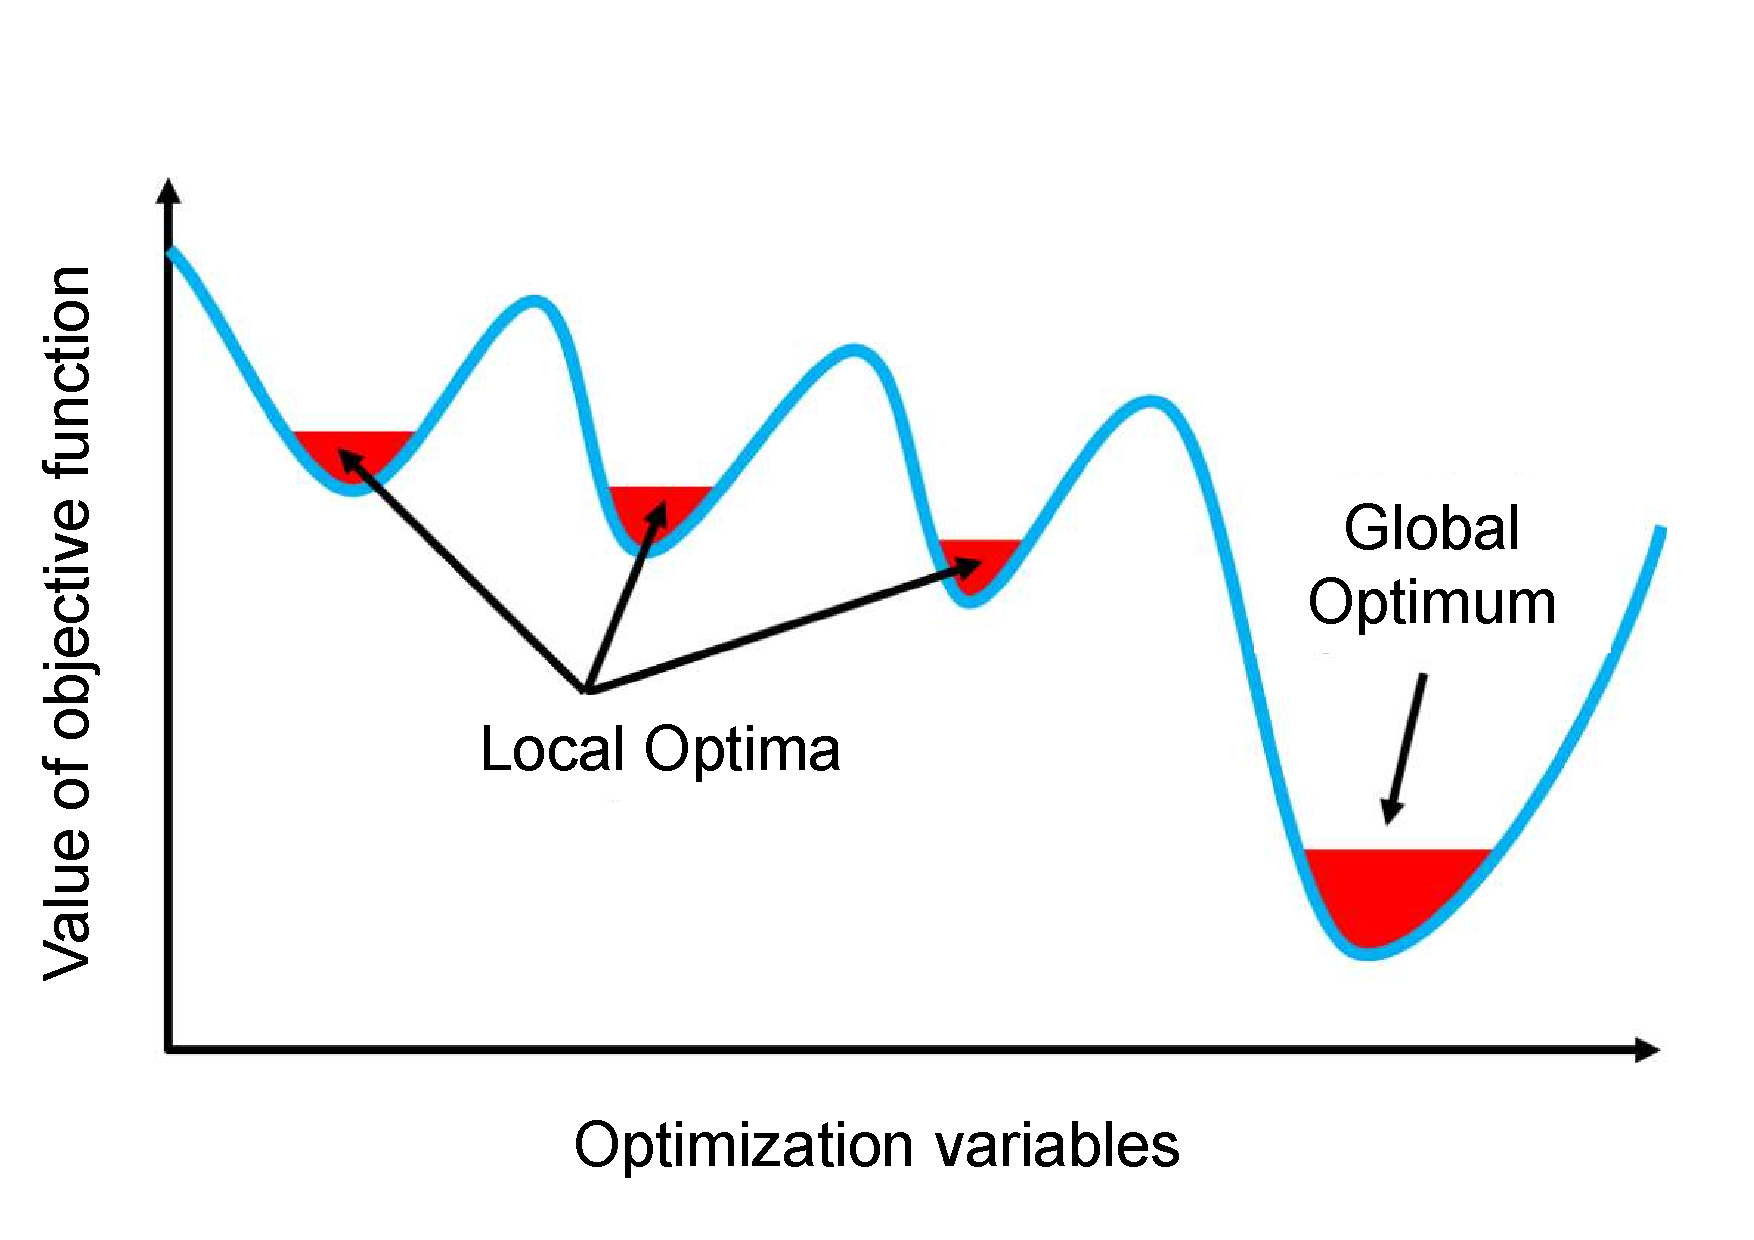
\includegraphics[width=10cm]{03_images/local_global.pdf}
	\caption{Difference between local and global optimum}
	\label{fig:Introduction:local_global}
\end{figure}
Depending on the end effector stiffness, there can be multiple local extremum points in an objective function. In the optimization process, it is likely that the decision variables stay around those points and cannot progress towards a pole, as shown in Figure \ref{fig:Introduction:local_global}. Finding the global optimum is the goal, while the local optimum is not the ideal result. As shown in Figure \ref{fig:Introduction:local1} and Figure \ref{fig:Introduction:local2}, there are several local optima. If the variables change a bit, the objective function results in a higher value, but the optimization process may find the global optimum when the variables change a lot.\par
\begin{figure}[h!]
\centering
\vspace{-0.7cm}
\setlength{\abovecaptionskip}{-0.1cm} 
\begin{minipage}[t]{0.48\textwidth}
\centering
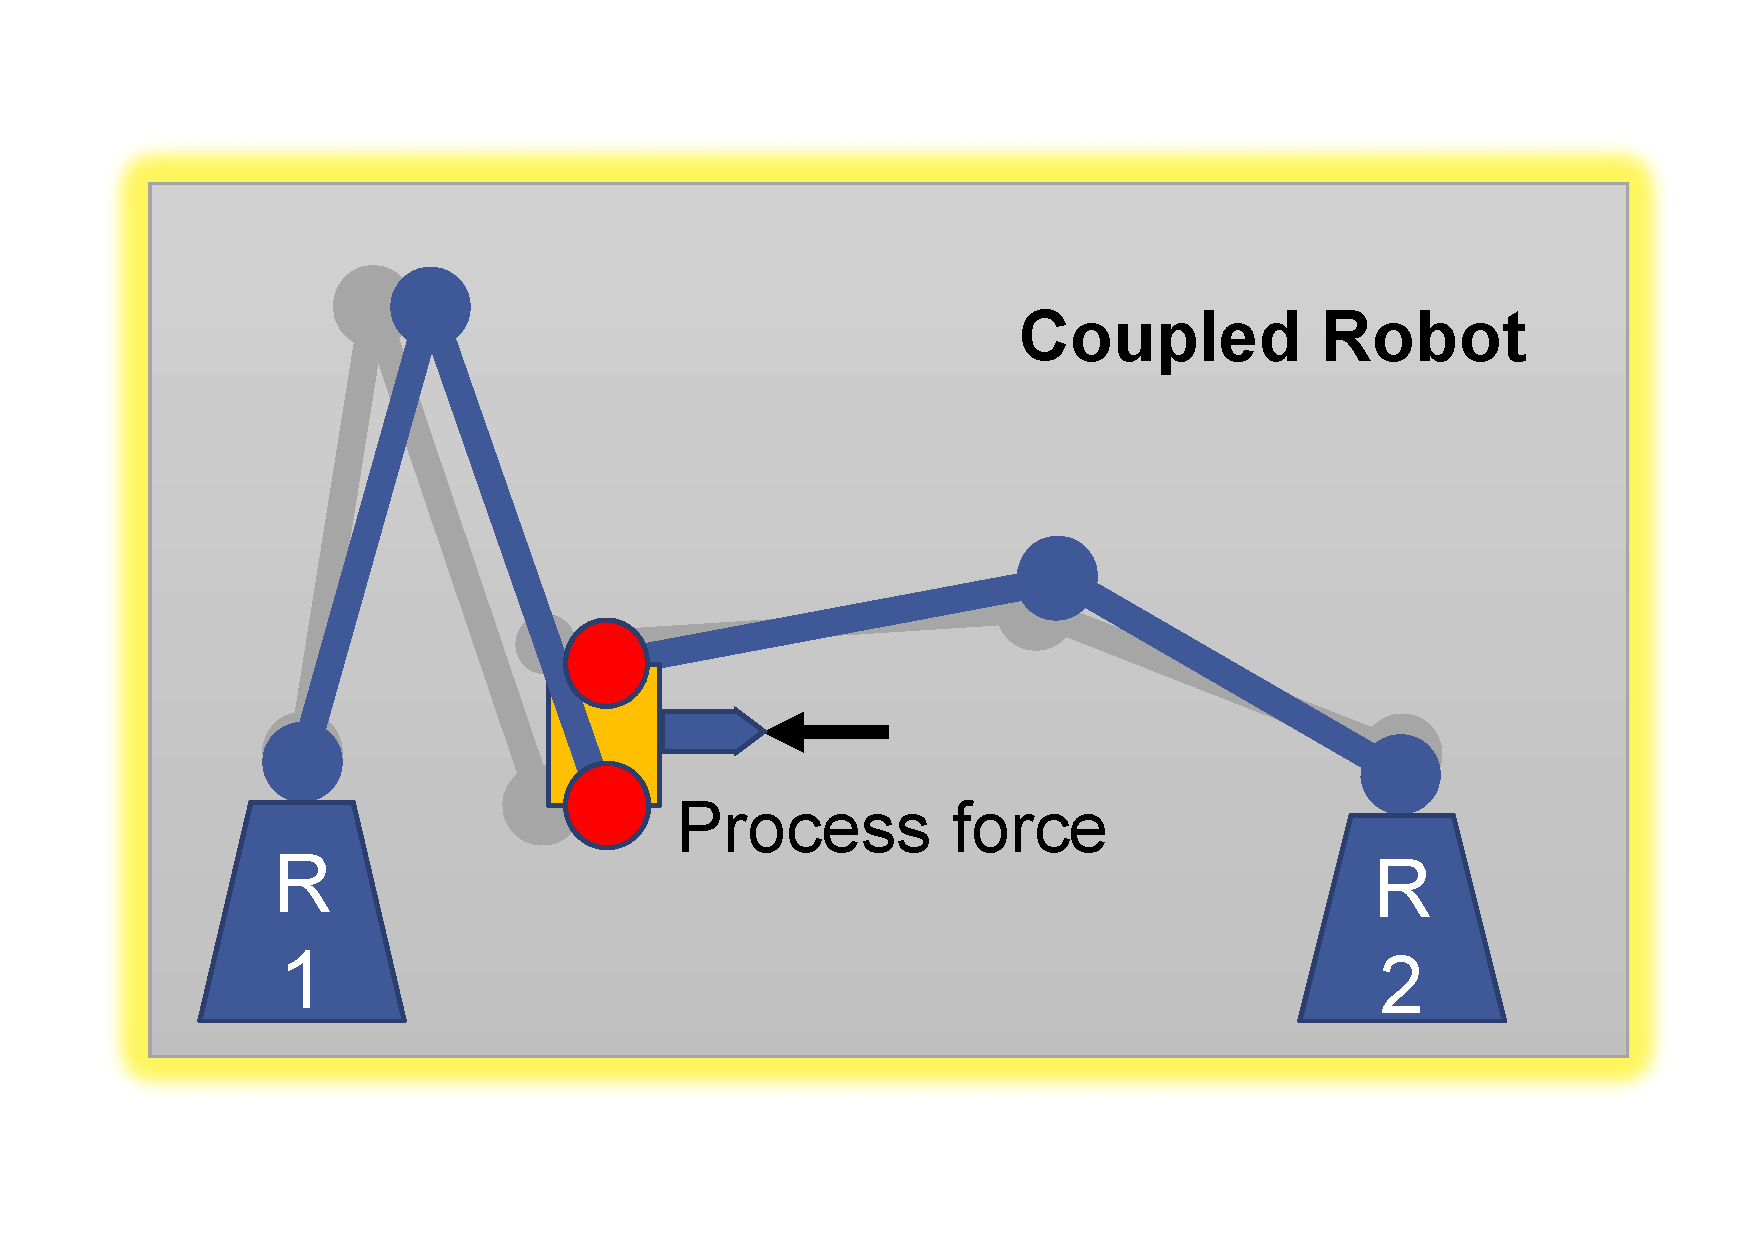
\includegraphics[width=6cm]{03_images/local1.pdf}
\caption{Local 1}
\label{fig:Introduction:local1}
\end{minipage}
\begin{minipage}[t]{0.48\textwidth}
\centering
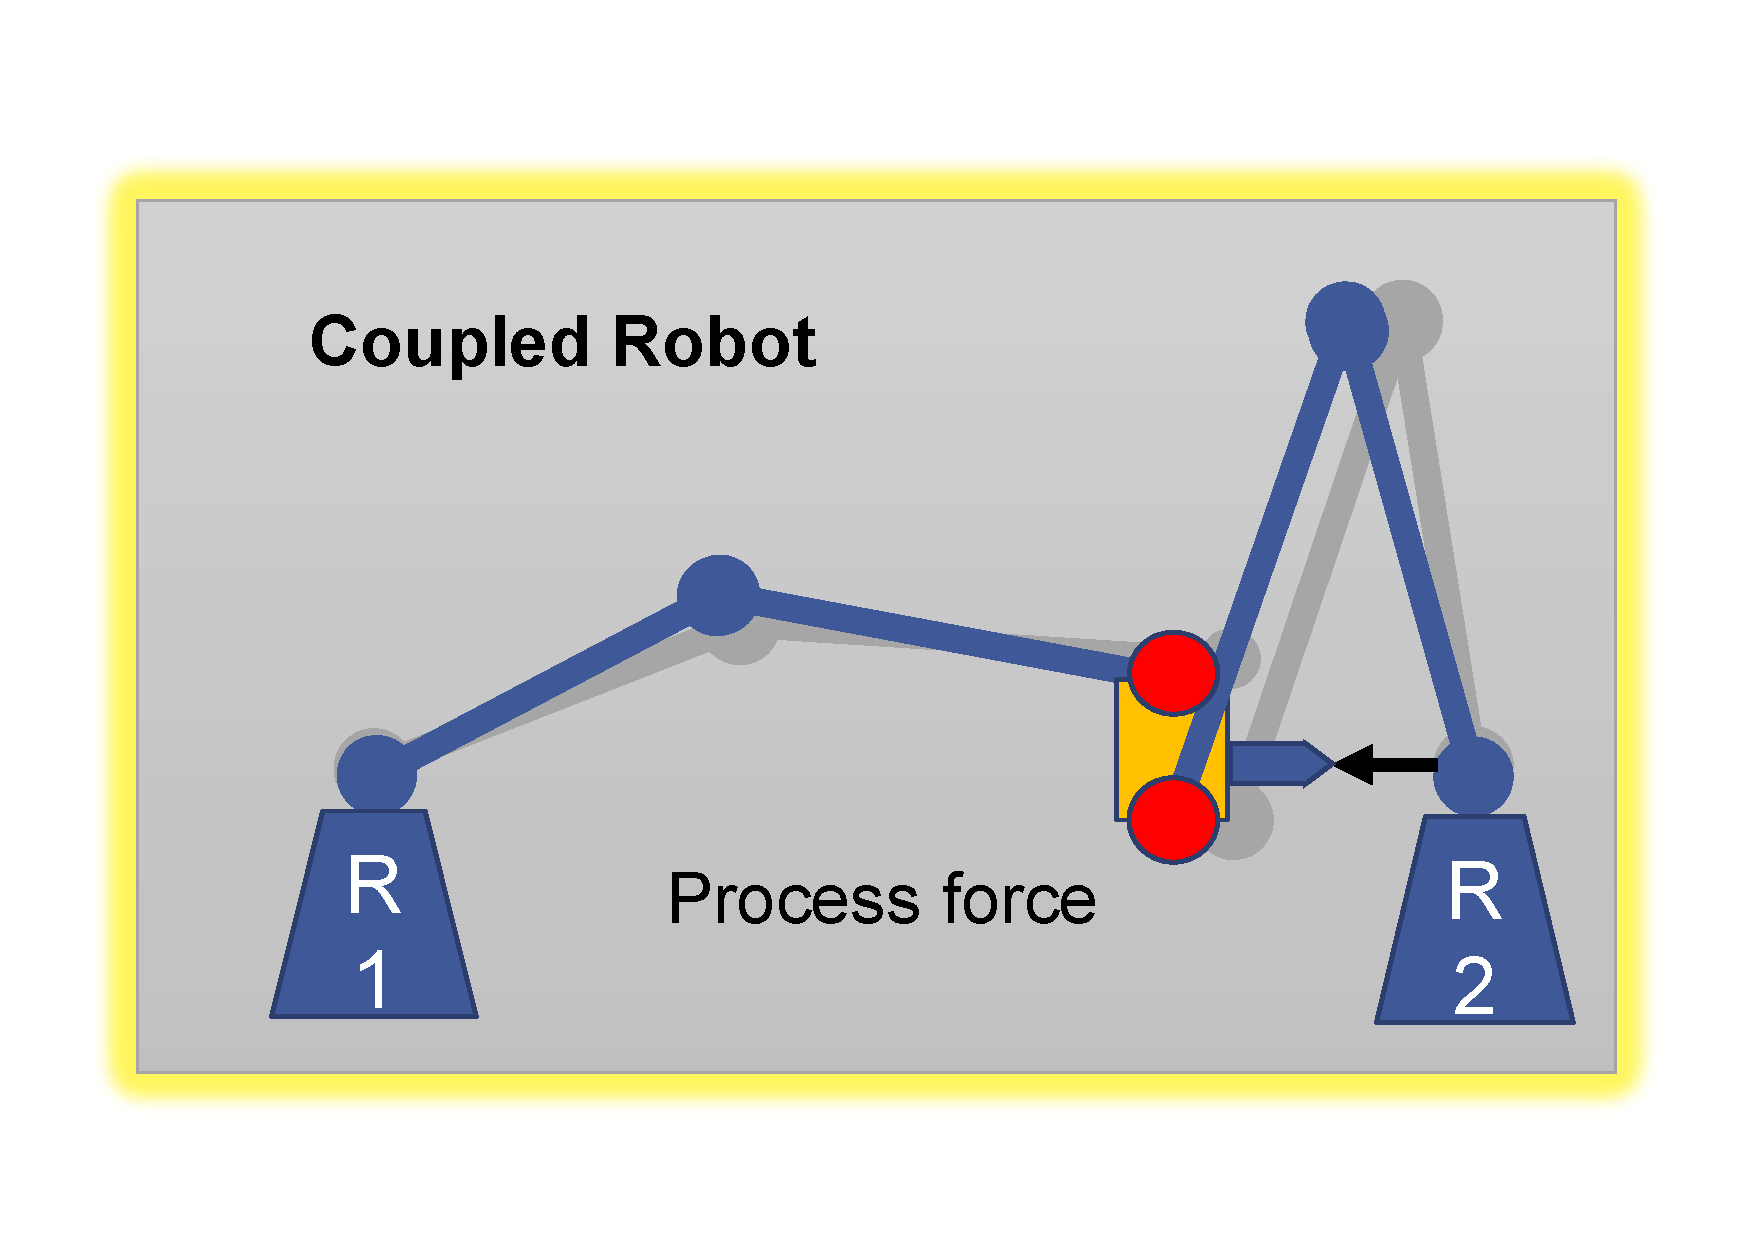
\includegraphics[width=6cm]{03_images/local2.pdf}
\caption{Local 2}
\label{fig:Introduction:local2}
\end{minipage}
\vspace{-0.5cm}
\end{figure}
Since the goal of the thesis is action planning to enhance stiffness for coupled industrial robots in manufacturing processes, an optimization method is needed to find the global optimum stiffness of the joint angle configuration of the coupled robot and the corresponding placement of the workpiece.\par
As the final goal of enhancing the stiffness is to improve the machining accuracy of the workpiece, moving the robot during machining can reduce the accuracy due to position errors. Similarly, moving the robot during machining is inconvenient and requires the coupler to be disassembled before it can be assembled and calibration. So the placement of the two robots is fixed during the machining process.\par
So the optimization variables are the joint angle configuration of the coupled robot and the corresponding position of the workpiece:\par
(1)The joint angle configuration of the coupled robot is as follows: 
\begin{equation}
  \boldsymbol{\theta} =  \left[ \theta_{1},\theta_{2},...,\theta_{n} \right]^\top \in \mathbb{R}^{n} 
\end{equation}
$n$ represents the total joint number of the coupled robot.\par
(2)The placement of the workpiece is as follows:
\begin{equation}
\boldsymbol{s} =  \left[x,y,z,\alpha,\beta,\gamma\right]^\top \in \mathbb{R}^{6}
\end{equation}
$x$ represents the position of the workpiece in the x-axis direction, $y$ represents the position of the workpiece in the y-axis direction, $z$ represents the position of the workpiece in the z-axis direction, $\alpha$ represents the angle of rotation of the workpiece in the x-axis direction, $\beta$ represents the angle of rotation of the workpiece in the x-axis direction, and $\gamma$ represents the angle of rotation of the workpiece in the x-axis direction.\par
After defining the goal of thesis, it is first necessary to identify the relevant constraints.\par
(a)The coupled robot needs to move along a predefined machining path to ensure that the actual machining path matches the predefined path, in which the path is on the workpiece and can be placed freely in the space.\par
(b)As the two robots are coupled together utilizing a rigid connector, the optimization process ensures that the end connectors of the two robots are permanently coupled, i.e., the end-effectors of two robots are in the same position.\par
(c)In addition, the angle of the robot joints must not be exceeded during machining.\par
Finally, the objective function needs to be determined as follows:
\begin{equation}
\mathcal{J} = \mathcal{J}\left(\boldsymbol{\theta},\boldsymbol{s}\right)
\end{equation}
$\boldsymbol{\theta}$ represents the joint angle configuration of the coupled robot, and $\boldsymbol{s}$ represents the placement of the workpiece.
\section{System structure for the optimization of stiffness} \label{sec:Introduction:System structure}
\begin{figure}[h!]
	\centering
        \setlength{\abovecaptionskip}{-3cm} 
	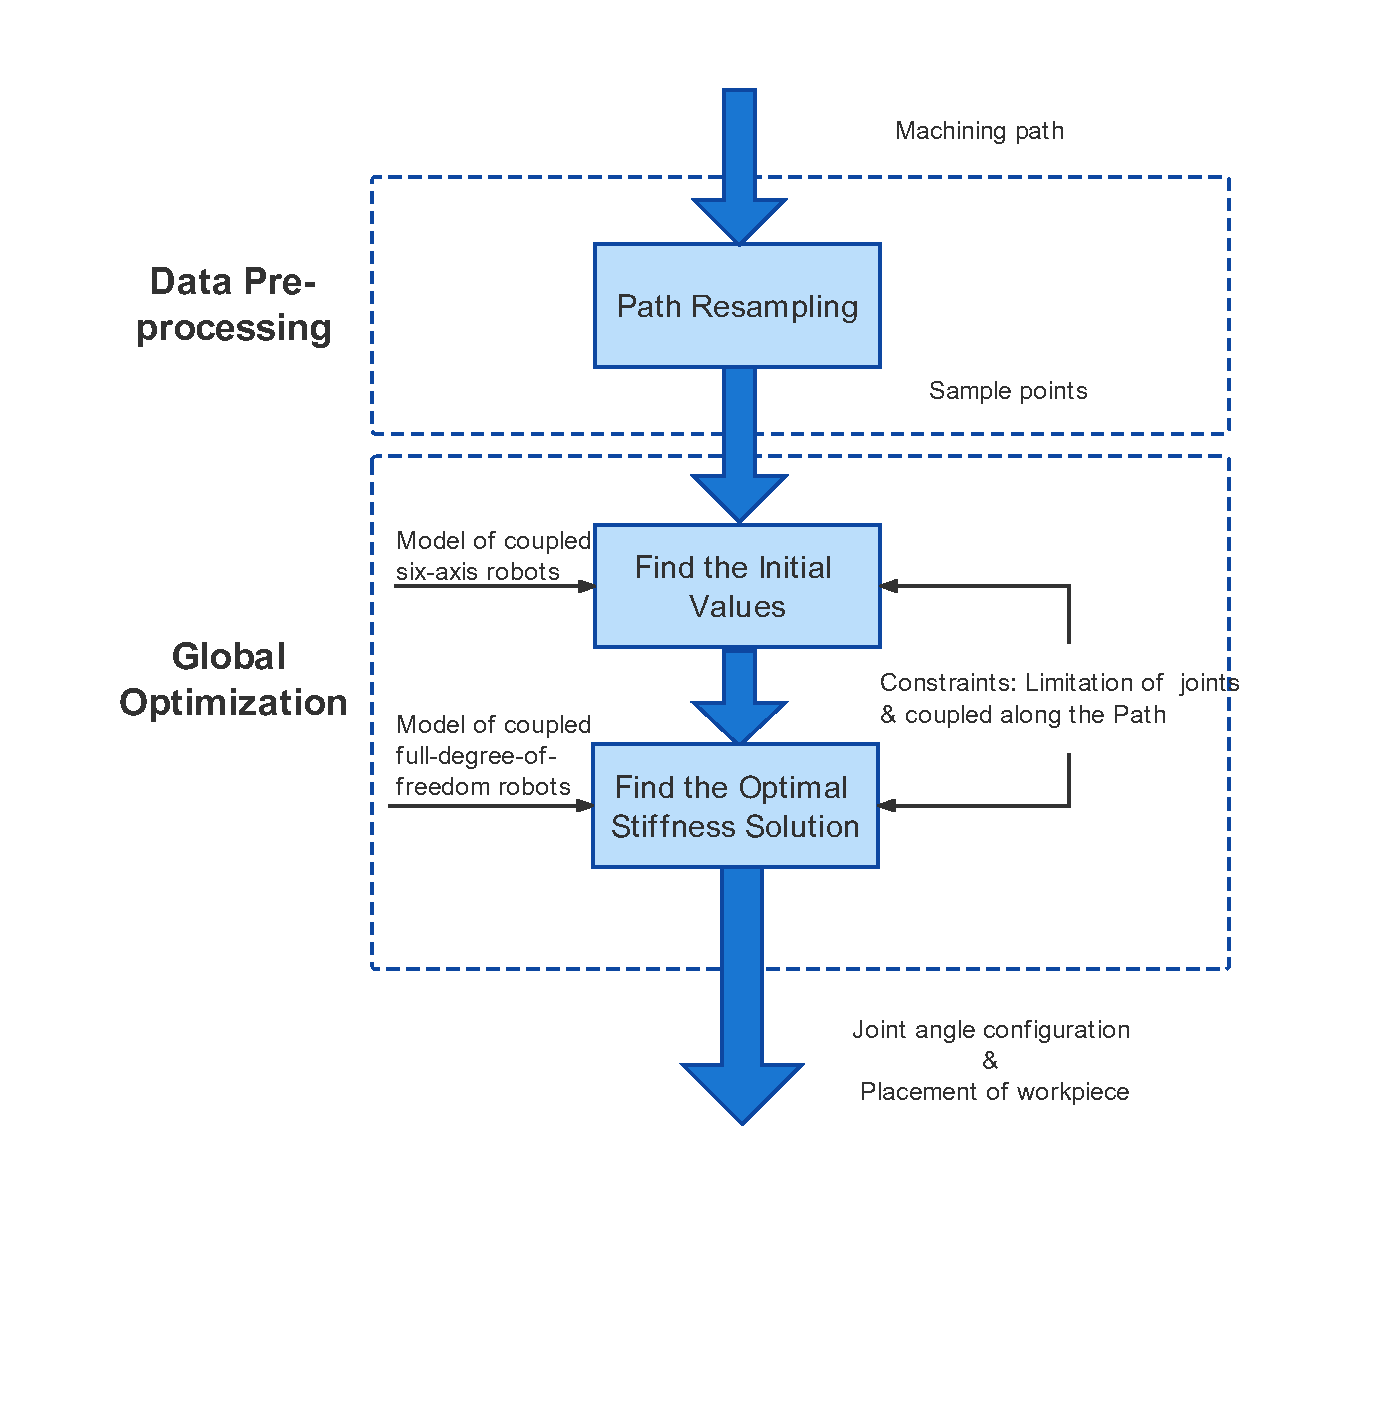
\includegraphics[width=\textwidth]{03_images/pipeline_full.pdf}
	\caption{System structure diagram}
	\label{fig:Introduction:pipeline}
\end{figure}
Figure \ref{fig:Introduction:pipeline} shows the steps required to optimize the stiffness system, it consists of data pre-processing and the global optimization.The input of this system is the intended machining path, and the output is the joint angle configuration of the coupled robot and the corresponding placement of the workpiece.\par
In order to solve the above problem and satisfy the constraint (a), tracking a continuous machining path is time-consuming and computationally intensive, so data pre-processing is needed. This machining path is fixed and given input into the planning system. Some points characterizing the whole course of the machining path without much loss of information about the straight and curving parts need to be found, and these points are the so-called sample points. \par
The goal is to find the joint angle configuration of the coupled robot and the corresponding position of the workpiece for the global optimum stiffness. The whole model is highly customized. Apart from the robots which are available in the Matlab robotics toolbox, it also consists of the couple module and the workpiece placement. Therefore, it is essential to build a model that contains both the coupled robots and the placement of the workpiece.\par
In the global optimization process, a global optimization method needs to be used to optimize the stiffness, which achieves the goal of going out of the local optimum of stiffness and continuing the search for the global optimum.\par
Finding good initial values is significant to finding the global optimum solution faster, so initial values generated respecting the constraint conditions rather than randomly. So a method of finding the initial function needs to be chosen. There is a function in the Matlab toolbox that can be used to solve closed-form inverse kinematics \cite{AIK}, but it only supports a six-degree-of-freedom robot model, so a six-degree-of-freedom model need to build.\par
In order to find the optimal stiffness solution, a coupled full degree of freedom robot model needs to be modeled. Compared with the general six-degree-of-freedom robot, the seven-degree-of-freedom robot has one more degree of freedom, which allows it to change its configuration while keeping the end pose unchanged, achieving obstacle avoidance, avoiding joint limiting, avoiding singularity, and reducing joint torque consumption. The KUKA iiwa LBR 14 R820 robot \cite{kuka_datasheet} is a typical seven-degree-of-freedom robot chosen to be used in the following thesis. Since the robot used is the KUKA iiwa LBR 14 R820, which has seven-degree-of-freedom as figure \ref{fig:Introduction:kuka} shows, the six-degree-of-freedom model is not applicable here, so a coupled full-degree-of-freedom robot model is needed.\par
\begin{figure}[h!]
	\centering
	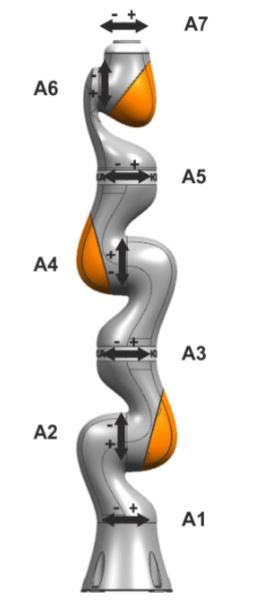
\includegraphics[scale=1]{03_images/kuka_7.JPG}
	\caption{KUKA iiwa LBR 14 R820 robot}
	\label{fig:Introduction:kuka}
\end{figure}
During the global optimization process, it is necessary to ensure that two or more robots are coupled and travel along the pre-defined machining path while satisfying the limitation of the rotation angle of each joint.
\section{Purpose of the thesis} \label{sec:Introduction:Purpose}
This thesis aims to optimize the stiffness of the coupled robot during the machining process, while the three constraints (a)(b)(c) need to be satisfied.\par
The thesis aims to use global optimization methods that can overcome local optima and continue the search for the global optimum when optimizing the stiffness of a coupled robot.\par
The optimized stiffness reduces the joint angle load of the coupling robot due to machining forces during the machining process, which eventually increases the accuracy of the machined workpiece.\par
As the placement and joint angles are regarded as variables for optimization without explicit consideration of robot dynamics, the stiffness optimization should still be able to apply to real robots practically. It requires the robot to move smoothly along the machining path during the machining process, i.e., in addition to enhancing the stiffness, it also needs to avoid abrupt changes in joint angle when the coupled robots drive the end effector from one sample point of the predefined path to the other.
\section{Structure of the thesis} \label{sec:Introduction:Purpose}
After the background and motivation, problem definition, and purposes in this chapter, Chapter 2 discusses various optimization methods, including local and global optimization methods, heuristic and metaheuristic optimization methods, and their differences.
The different methods from the literature are explained and classified. The third chapter deals with how the selected global optimization methods can be used in the system to achieve optimization of the stiffness of the coupled robot during machining. In chapter
4, the results generated by the genetic algorithm and the particle swarm algorithm are compared and evaluated in simulations.In the final chapter 5, a summary and an outlook for future work are given.


















